\documentclass[11pt]{article}
\usepackage{mathrsfs}
\usepackage[centertags]{amsmath}
\usepackage{amsfonts}
\usepackage{amssymb}
\usepackage{amsthm}
\usepackage{cases}
\usepackage{indentfirst}
\usepackage{epsfig}
\usepackage {graphicx}
\usepackage{color}
\usepackage{CJK}


\parskip 1ex
\pagestyle{plain}
\oddsidemargin 0in
\topmargin 0.0in
\headheight 0in
\textwidth 6.5in
\textheight 9.0in
\date{}

\newtheorem{theorem}{Theorem}[section]
\newtheorem{corollary}{Corollary}[section]
\newtheorem{lemma}{Lemma}[section]
\newtheorem{condition}{Condition}[section]
\newtheorem{proposition}{Proposition}[section]
\newtheorem{remark}{Remark}[section]
\newtheorem{definition}{Definition}[section]
\numberwithin{equation}{section}
\renewcommand{\theequation}{\thesection.\arabic{equation}}
\def\P{\operatorname*{P}}
\def\E{\operatorname*{E}}
\def\Var{\operatorname*{Var}}
\def\Cov{\operatorname*{Cov}}
\def\sign{\operatorname*{sign}}
\def\R{\operatorname*{\mathbb{R}}}
\def\F{\operatorname*{\mathbb{F}}}
\allowdisplaybreaks[4]

%%%%%%%%%%%%%%%%%%%%%%%%%%%%%%%%%%%%%%%%%%%%%%%%%%%%%%%%%%%%%
\begin{document}
\title{\textbf{Tests of inflated zeros for \\ censored Poisson regression model}}
\maketitle

%%%%%%%%%%%%%%%%%%%%%%%%%%%%%%%%%%%%%%%%%%%%%%%%%%%%%%%
\section{Models}
\label{sec1}

%%%%%%%%%%%%%%%%%%%%%%%%%%%%%%%%%%%%%%%%%%%%%%%%%%%%%%%%%%
\subsection{Poisson Model} \label{sec1-1}

Poisson Regression:
            \:\:$Y_i|X_i \sim i.d. \:\: \mbox{Poisson}(\mu_i),\:\: \log(\mu_i)=x_i^T\beta$

Poisson Model:
            \:\:$P(Y_i=y_i)=\frac{e^{-\mu_i}\mu_i^{y_i}}{y_i!},\:\: y_i \ge 0$

%%%%%%%%%%%%%%%%%%%%%%%%%%%%%%%%%%%%%%%%%%%%%%%%%%%%%%%%%%
\subsection{ZIP Model} \label{sec1-2}
ZIP Regression:\:\:$Y_i|X_i \sim i.d. \:\: \mbox{ZIP}(\omega_i,\mu_i),\:\:\ \mbox{logit}(\omega_i)= u^T_i \beta_{\omega},\:\: \log(\mu_i)=x^T_i\beta_{\mu}$

ZIP Model:
\begin{align}
P(Y_i=y_i)=\left\{
                \begin{array}{cc}
                    \omega+(1-\omega)e^{-\mu_i}, & y_i=0 \\
                    (1-\omega)\frac{e^{-\mu_i}\mu_i^{y_i}}{y_i!},  & y_i>0
                \end{array}
            \right. 
\end{align}

%%%%%%%%%%%%%%%%%%%%%%%%%%%%%%%%%%%%%%%%%%%%%%%%%%%%%%%%%%
\subsection{Censored Poisson Model} \label{sec1-3}
Censored Poisson Regression:

\begin{align}
     &Y_i| X_i \sim i.d. \mbox{Poisson}(\mu_i)  \nonumber\\
     &Z_i = \min\left\{Y_i,L\right\}=\left\{
                \begin{array}{cc}
                    y_i &,y_i < L  \\
                    L&,y_i \ge L
                \end{array} \right.;\nonumber\\
     &Z_i | X_i \sim i.d. \:\: \mbox{CensoredPoisson}(\mu_i,L),\:\: \log(\mu_i)=x_i^T\beta 
\end{align}




Censored Poisson Model:
\begin{align}
    P(Z_i=z_i) &= P \left\{ \min(Y_i,L)=z_i \right\} \nonumber\\
                &=\left\{
                    \begin{array}{ccc}
                        P(Y_i = z_i)&, z_i<L \nonumber\\
                        P(Y_i \ge L)&,z_i = L \nonumber\\
                        0&,z_i > L
                    \end{array}
                 \right.\\
             &=\left\{  \begin{array}{ccc}
                        \frac{e^{-\mu_i}\mu_i^{z_i}}{z_i!}&,0\le z_i<L \\
                        \sum_{y_i=L}^{\infty}{P(Y_i=y_i)}&,z_i = L \\
                        0&,z_i > L
                        \end{array}    \right.
\end{align}

                       

Likelihood function of censored Poisson:
\begin{align}
            &d_i = I_{(z_i\ge L)} \nonumber\\
            &c_i = P(Y_i\ge L)= \sum_{y_i=L}^{\infty}{P(Y_i=y_i)} \nonumber\\
            &L_1=\prod_{i=1}^n\left\{ \left[ \frac{e^{-\mu_i}\mu_i^{z_i}}{z_i!} \right]^{(1-d_i)} \left[  \sum_{y_i=L}^{\infty}{P(Y_i=y_i)}\right]^{d_i} \right\} 
\end{align}

Log-likelihood function of censored Poisson:
\begin{align}
            l_1=log(L_1)=
                \sum_{i=1}^n\left\{(1-d_i)log\left[ \frac{e^{-\mu_i}\mu_i^{z_i}}{z_i!} \right]
                + d_i log (c_i) \right\}  
\end{align}
%%%%%%%%%%%%%%%%%%%%%%%%%%%%%%%%%%%%%%%%%%%%%%%%%%%%%%%%%%
\subsection{Censored ZIP Model} \label{sec1-4}
Censored ZIP Regression:
\begin{align}
            &Y_i| X_i \sim i.d. \:\: \mbox{ZIP}(\omega_i,\mu_i) \nonumber\\
            &Z_i = \min\left\{Y_i,L\right\}=\left\{
                    \begin{array}{cc}
                        y_i &,y_i < L  \nonumber\\
                        L&,y_i \ge L
                    \end{array}   \right.  \nonumber\\
             &Z_i | X_i \sim i.d. \:\: \mbox{CensoredZIP}(\omega_i,\mu_i,L), \:\: \mbox{logit}(\omega_i)=u_i^T\beta_{\omega}
                     ,\:\: \log(\mu_i)=x_i^T\beta_{\mu}  
\end{align}
Censored ZIP Model:
\begin{align}
            P(Z_i=z_i) &= P \left\{ min(Y_i,L)=z_i \right\}\nonumber\\
            &=\left\{
                    \begin{array}{ccc}
                        P(Y_i = z_i)&,  z_i<L \nonumber\\
                        P(Y_i \ge L)&, z_i = L \nonumber\\
                        0&, z_i>L
                    \end{array}    \right.  \nonumber\\
            &=\left\{
                    \begin{array}{ccc}
                            \omega+(1-\omega)P(Y_i = 0) &,  z_i = 0 \\
                            (1-\omega)P(Y_i = z_i) &, 0< z_i<L \\
                         (1-\omega)\sum_{y_i=L}^{\infty}{P(Y_i=y_i)} & z_i = L\\
                        0 &,z_i>L
                    \end{array}
                 \right. \nonumber\\
            &=\left\{
                    \begin{array}{ccc}
                            \omega+(1-\omega)e^{-\mu_i} &,  z_i = 0 \\
                            (1-\omega)\frac{e^{-\mu_i}\mu_i^{z_i}}{z_i!} &, 0< z_i<L \\
                         (1-\omega)\sum_{y_i=L}^{\infty}{P(Y_i=y_i)} & z_i = L \\
                        0 &,z_i>L
                    \end{array}
                 \right.
\end{align}
Likelihood function of censored ZIP model:
\begin{align}
            &r_i = I_{(z_i=0)} \nonumber\\
            &d_i = I_{(z_i\ge L)} \nonumber\\
            &c_i = P(Y_i\ge L)= \sum_{y_i=L}^{\infty}{P(Y_i=y_i)} \nonumber
\end{align}

\begin{align}
            L_2 = \prod_{i=1}^n \left\{
                                    \left[(1-\omega) \sum_{y_i=L}^{\infty}{P(Y_i=y_i)} \right]^{d_i}
                                    \left[
                                            \left( \omega+(1-\omega)e^{-\mu_i} \right)^{r_i}
                                            \left((1-\omega)\frac{e^{-\mu_i}\mu_i^{z_i}}{z_i!}\right)^{1-r_i}
                                    \right]^{1-d_i}
                                \right\} \nonumber
\end{align}


Log-likelihood function of censored ZIP model:
\begin{align}
            l_2=log(L_2)
            = \sum_{i=1}^n \left\{
                (1-d_i) \left[
                \left( r_i \bullet log(\omega +(1-\omega)e^{-\mu_i}) \right)
                + (1-r_i)log\left(   \left(1-\omega \right)
                                  \left(\frac{e^{-\mu_i}\mu_i^{z_i}}{z_i!}\right)   \right)
                            \right]
\notag\right.
\\
\phantom{=\;\;}
\left.
                + d_i \bullet log((1-\omega)\bullet c_i))
            \right\} \nonumber
\end{align}


%%%%%%%%%%%%%%%%%%%%%%%%%%%%%%%%%%%%%%%%%%%%%%%%%%%%%%%
\section{Hypothesis}
\label{sec2}
$$H_0:\omega = 0\:\:\: vs.\:\:\:H_1:\omega > 0$$


%%%%%%%%%%%%%%%%%%%%%%%%%%%%%%%%%%%%%%%%%%%%%%%%%%%%%%%
\section{Test}
\label{sec3}

%%%%%%%%%%%%%%%%%%%%%%%%%%%%%%%%%%%%%%%%%%%%%%%%%%%%%%%
\subsection{Wald Test}  \label{sec3-1}
Wald statistics:
        $$ \frac{\hat{\omega}}{\hat{\sigma}} \sim N(0,1) \:\:\:or\:\:\: \frac{\hat{\omega}^2}{\hat{\sigma}^2} \sim \chi^2(1)$$

Method:

from MLE of the CZIP we can get $\hat{\omega}$ ;
then use Fisher Information matrix to get estimate the var of $\hat{\omega}$;
that we have Wald statistics $\frac{\hat{\omega}^2}{\hat{\sigma}^2}$ and it follows $\chi^2(1)$.

%%%%%%%%%%%%%%%%%%%%%%%%%%%%%%%%%%%%%%%%%%%%%%%%%%%%%%%
\subsection{LR Test}  \label{sec3-2}
LR statistics:
$$ S_{LR}=2\left[ l_2(\hat{\omega},\hat{\beta})- l_1(0,\hat{\beta}) \right]\sim \chi^2(1)
$$

%%%%%%%%%%%%%%%%%%%%%%%%%%%%%%%%%%%%%%%%%%%%%%%%%%%%%%%%
\subsection{Score Test}  \label{sec3-3}
Score statistics:
            $$ S_{score}\sim N(0,1) $$

Method:
let$\theta = \frac{\omega}{1-\omega}$;
then from MLE of the CZIP we can get$\hat{\theta},\hat{\beta}$;
then let $\theta =0$equaling to $\omega=0$, so we have $\hat{\theta_0}$;
then use Fisher Information matrix to get estimate the var of$\hat{\theta_0}$ ;
that we have Score statistics$ \frac{\hat{\theta_0}}{\sigma_{\theta_0}}\sim N(0,1)$.

Details:

Firstly,$\theta = \frac{\omega}{1-\omega}$,$p_i=e^{-\mu_i}$;

Then, from MLE of the CZIP we can get $\hat{\theta},\hat{\beta}$;
\begin{align}
               &\frac{\partial{l_2}}{\partial{\theta}}=\sum_{i=1}^n \left\{ \frac{-1}{\theta+1} + (1-d_i)
                  \left[\frac{r_i}{\theta+p_i} \right]
                 \right\} \\
                &\frac{\partial{l_2}}{\partial{\beta}}=\sum_{i=1}^n \left\{(1-d_i)\left[
                \frac{-r_i\mu_i p_i x_i^T}{\theta_i +  p_i}
                +(1-r_i)(z_i-\mu_i)x_i^T\right]
                +\frac{d_i}{c_i}\frac{\partial{c_i}}{\partial{\beta}} \right\} 
\end{align}
and,
\begin{align}
            \frac{\partial{c_i}}{\partial{\beta}}&=
            \frac{\partial{\sum_{y_i=L}^{\infty}{P(Y_i=y_i)}}}{\partial{\beta}} \\
            &=\frac{\partial{\left[1-\sum_{y_i=0}^{L-1}{P(Y_i=y_i)}\right]}}{\partial{\beta}} \nonumber\\
           &=-\sum_{y_i=0}^{L-1}\frac{\partial{{P(Y_i=y_i)}}}{\partial{\beta}} \nonumber\\
           &=-\sum_{y_i=0}^{L-1}\frac{\partial{{\frac{e^{-\mu_i}\mu_i^{y_i}}{(y_i)!}}}}{\partial{\beta}} \nonumber\\
           &=-\sum_{y_i=0}^{L-1}(y_i-\mu_i)P(Y_i=y_i)x_i^T \nonumber\\
           &=\mu_i\sum_{k=0}^{L-1}P(Y_i=y_i)-y_i\sum_{k=0}^{L-1}P(Y_i=y_i) \nonumber\\ &=\mu_i\sum_{k=0}^{L-1}P(Y_i=y_i)-\mu_i\sum_{k=0}^{L-2}P(Y_i=y_i)\nonumber\\
        &=\mu_iP(Y_i=L-1)
\end{align}
So,
\begin{align}
            \frac{\partial{l_2}}{\partial{\beta}}=\sum_{i=1}^n \left\{(1-d_i)\left[
            \frac{-r_i\mu_i p_i}{\theta_i +  p_i}
            +(1-r_i)(z_i-\mu_i)\right]
            +\frac{d_i}{c_i}\mu_iP(Y_i=L-1) \right\}x_i^T
\end{align}

Then let $\theta=0$,
\begin{align}
            \frac{\partial{l_2}}{\partial{\theta}}|_{\theta=0}&=\sum_{i=1}^n \left\{
             \frac{(1-d_i)r_i-p_i}{p_i} \right\} \\
             \frac{\partial{l_2}}{\partial{\beta}}|_{\theta=0}&=\sum_{i=1}^n \left\{(1-d_i)\left[
            -r_i\mu_i
            +(1-r_i)(z_i-\mu_i)\right]
            +\frac{d_i}{c_i}\mu_iP(Y_i=L-1) \right\}x_i^T
\end{align}

Next, use Fisher Information matrix to get estimate the var of$\hat{\theta_0}$ . Finally, we have Score statistics $ \frac{\hat{\theta_0}}{\sigma_{\theta_0}}\sim N(0,1)$.


%%%%%%%%%%%%%%%%%%%%%%%%%%%%%%%%%%%%%%%%%%%%%%%%%%%%%%%%
\subsection{He Test}  \label{sec3-4}
He statistics:
\begin{align}
             \sqrt{n} \left( \hat{s} - 0 \right) \to N(0,\tau^2) 
\end{align}

 $\tau^2$ is (1,1)term of $A^{-1}BA^{-T}$  $(1,1)$;
 
 \begin{align}
 A(\gamma)&= E\left[ \frac{\partial}{\partial\gamma}\Psi_i( Y_i ,\gamma) \right] \\
  B(\gamma)&=Var(\Psi_i( Y_i ,\gamma)  
\end{align}
Details:
\begin{align}
E(r_i)&=P(z_i=0) \nonumber\\
&=P(Y_i=0) \nonumber\\
&=p_i  \\
s &=\frac{1}{n}\sum_{i=1}^n\left(r_i-E(r_i)\right)\nonumber\\
&=\frac{1}{n}\sum_{i=1}^n(r_i-p_i)
\end{align}
Estimation Equation(EE):
\begin{align}
            \psi _{1}&=\frac{1}{n}\sum_{i=1}^{n}\left( r_{i}-p_{i}-s\right)  \\
            \psi_{2}&=\frac{\partial{l_1}}{\partial{\beta}}=\frac{1}{n}\sum_{i=1}^{n}\left[(1-d_i)(z_i-\mu_i)+\frac{d_i}{c_i}\mu_iP(Y_i=L-1)\right] x_i^T  
\end{align}



%%%%%%%%%%%%%%%%%%%%%%%%%%%%%%%%%%%%%%%%%%%%%%%%%%%%%%%%
\section{Simulations}  \label{sec3-4}

\subsection{QQ plot Setting}
nism=100;n=c(50,100,200,500,1000);aa=c(-0.5,0.5,1,1.5)

case1:$\mu=e^{aa}$

case2:$\mu=e^{aa-1.45x},x\sim N(0,1)$

case3:$\mu=e^{aa-1.45x},x\sim U(0,1)$

cut=4:figure1,2,3;

cut=7:figure4,5,6;

cut=30:figure7,8,9;

\subsection{Power plot Setting}
nism=100;n=c(50,100,200,500,1000);aa=c(-0.5,0.5,1,1.5);lp=0.01*(seq(5,30,5))

case1:$\mu=e^{aa},\omega=lp$

case2:$\mu=e^{aa-1.45x},\omega=lp,x\sim N(0,1)$

case3:$\mu=e^{aa-1.45x},\omega=lp,x\sim U(0,1)$

cut=4:figure10,11,12;

cut=7:figure13,14,15;

cut=30:figure16,17,18;


\subsection{QQ plot}
\begin{figure}
  \centering
  % Requires \usepackage{graphicx}
  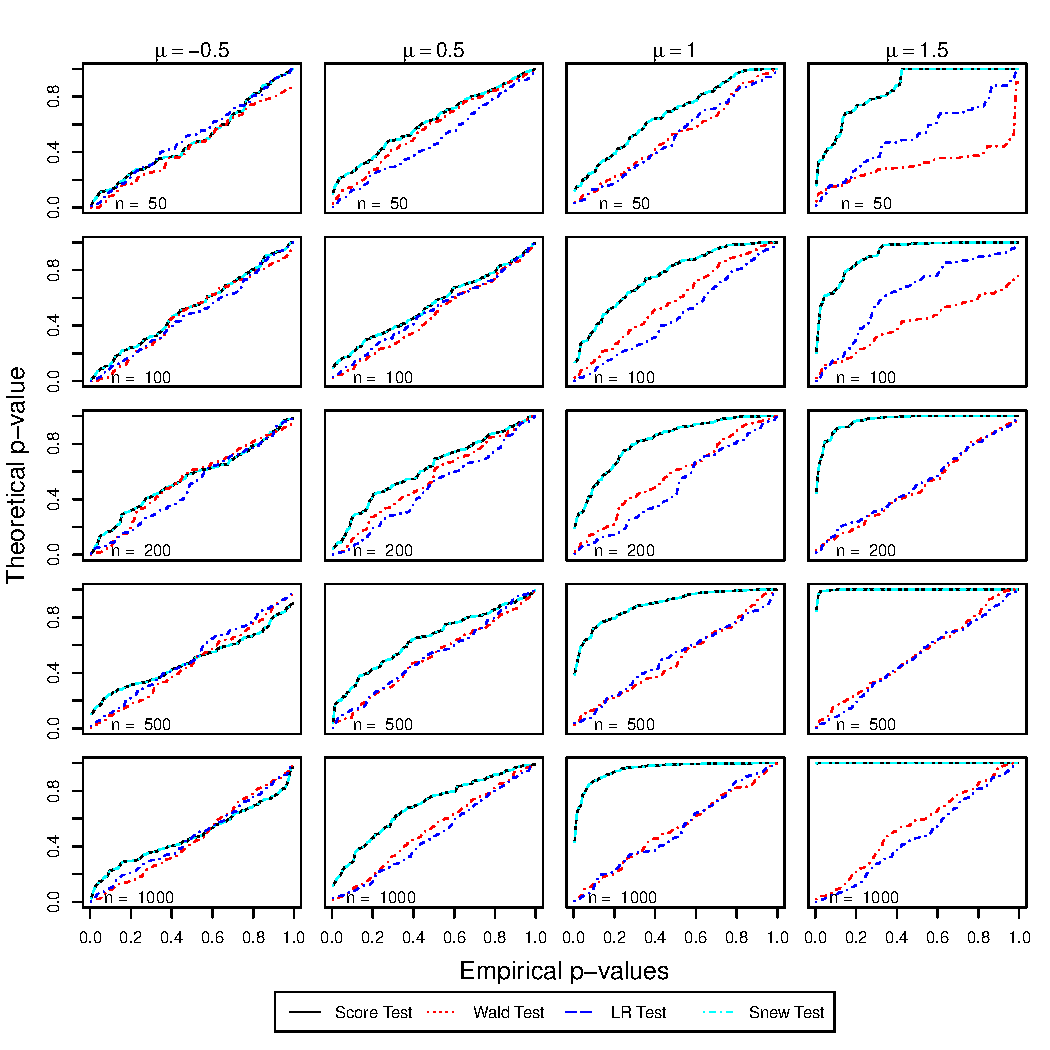
\includegraphics[width=\columnwidth]{./figure/q/q41.pdf}
  \caption{Power plot case1:$\mu=e^{aa}$;cut=4;}
\end{figure}

\begin{figure}
  \centering
  % Requires \usepackage{graphicx}
  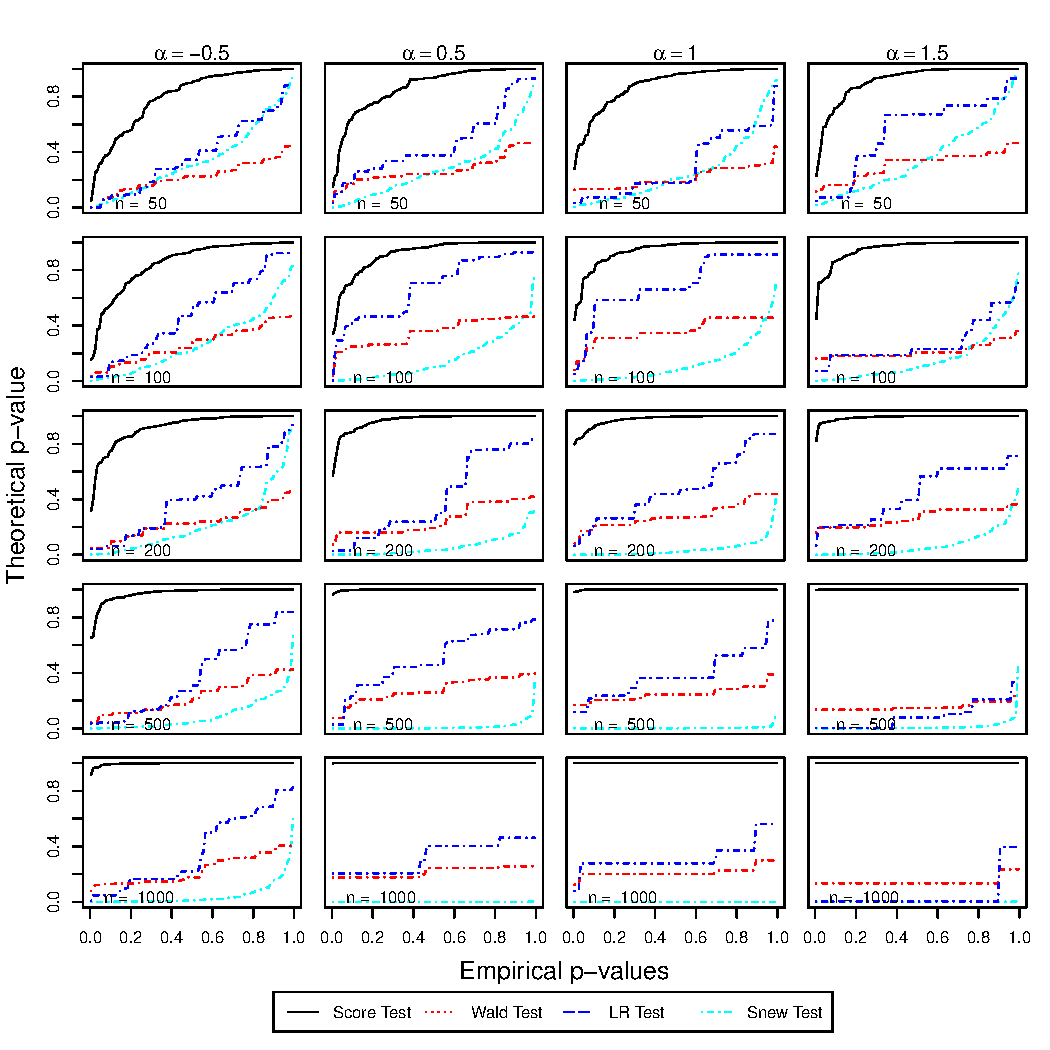
\includegraphics[width=\columnwidth]{./figure/q/q42.pdf}
  \caption{Power plot case2:$\mu=e^{aa-1.45x},x\sim N(0,1)$;cut=4}
\end{figure}

\begin{figure}
  \centering
  % Requires \usepackage{graphicx}
  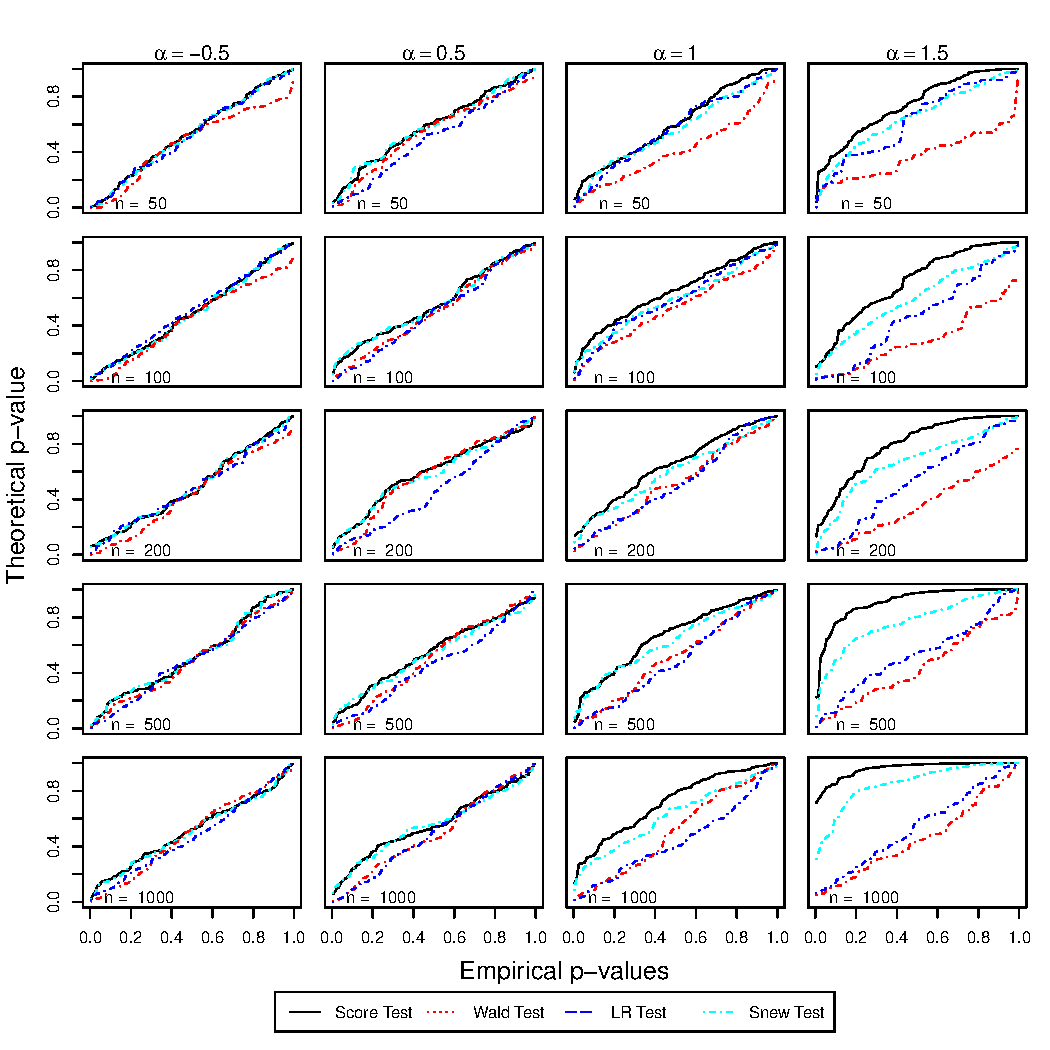
\includegraphics[width=\columnwidth]{./figure/q/q43.pdf}
  \caption{Power plot case3:$\mu=e^{aa-1.45x},x\sim U(0,1)$;cut=4}
\end{figure}

%%%%%%%%%%%%%%%%%%%%%%%%%%%%%%%%%%%%%%%%%%%%%%%%%%%%%%%%%%%%%%%%%%%%%%%%%%%%%%%%%%%

\begin{figure}
  \centering
  % Requires \usepackage{graphicx}
  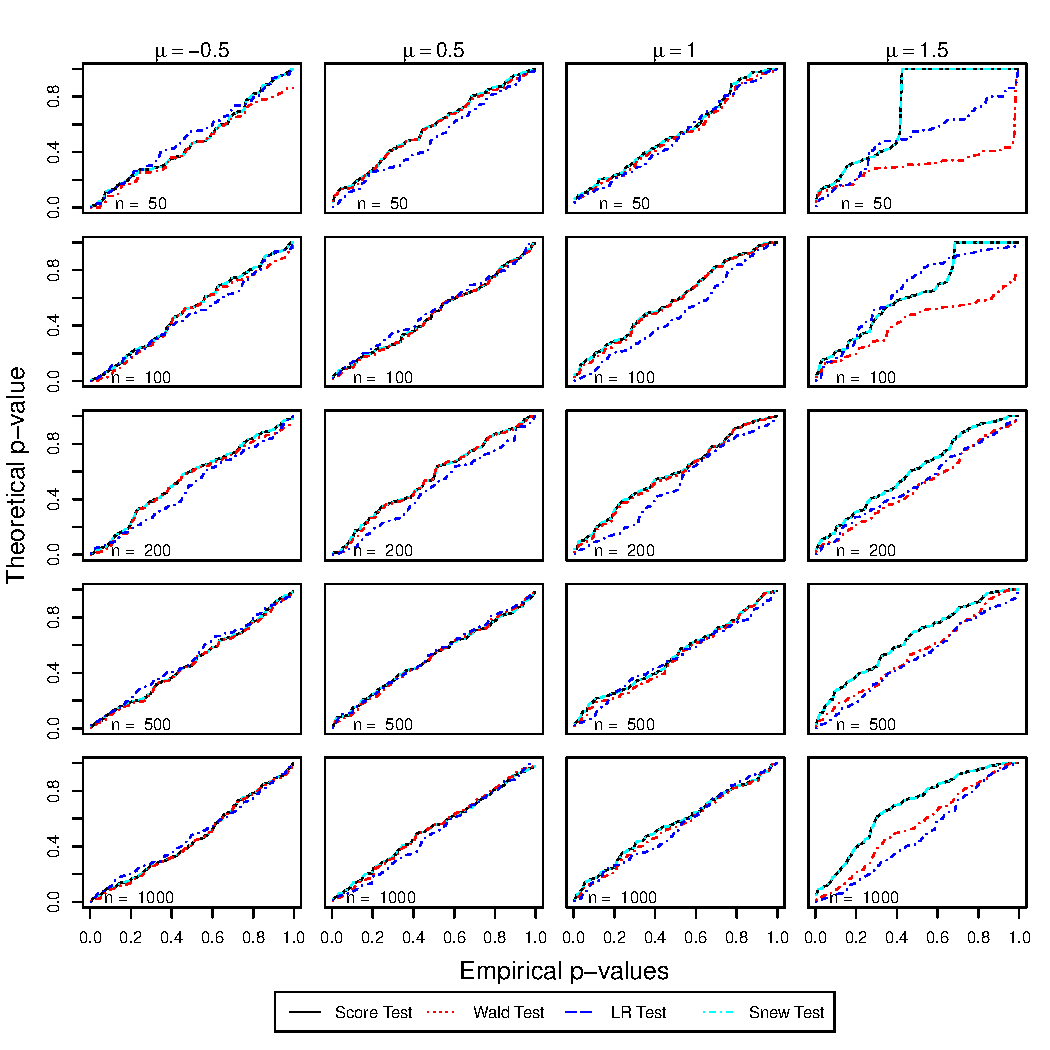
\includegraphics[width=\columnwidth]{./figure/q/q71.pdf}
  \caption{Power plot case1:$\mu=e^{aa}$;cut=7;}
\end{figure}

\begin{figure}
  \centering
  % Requires \usepackage{graphicx}
  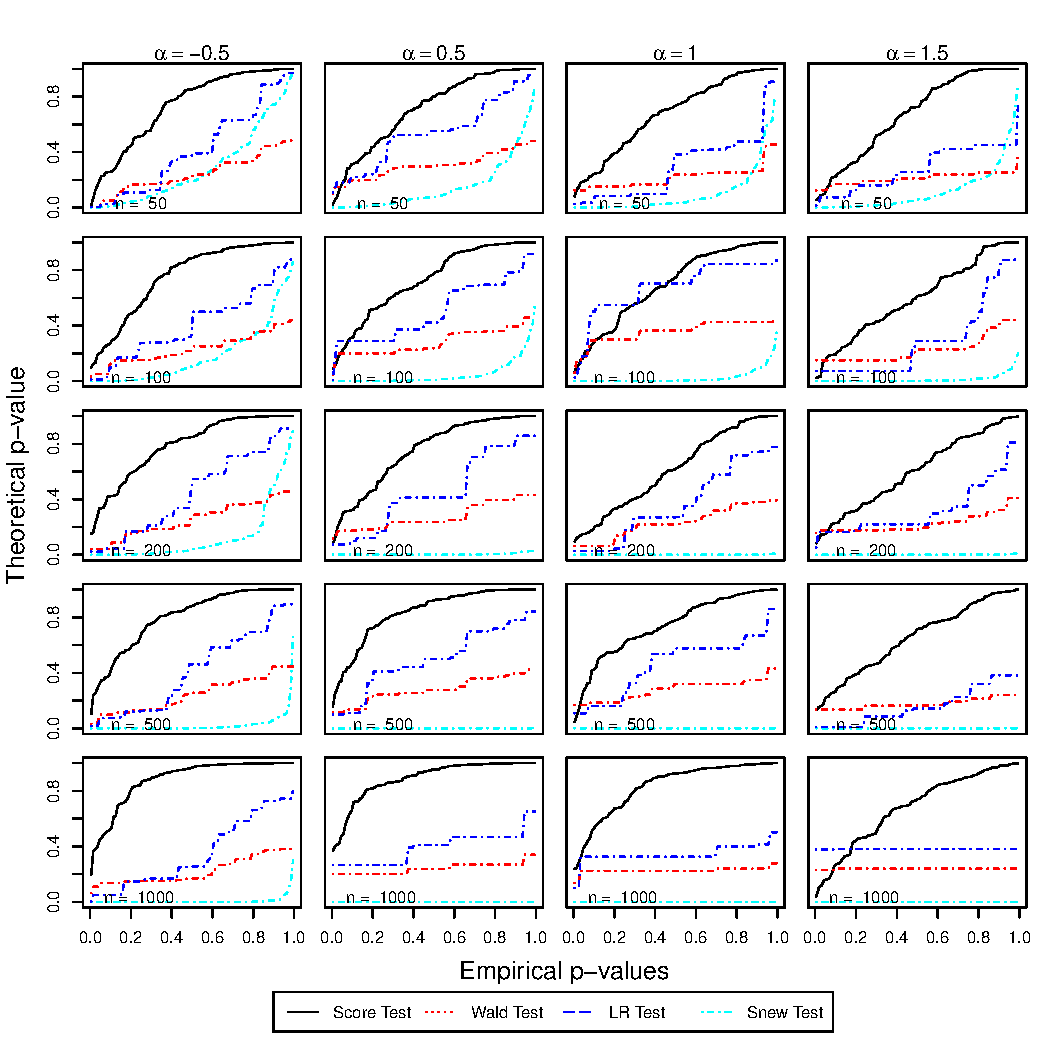
\includegraphics[width=\columnwidth]{./figure/q/q72.pdf}
  \caption{Power plot case2:$\mu=e^{aa-1.45x},x\sim N(0,1)$;cut=7}
\end{figure}

\begin{figure}
  \centering
  % Requires \usepackage{graphicx}
  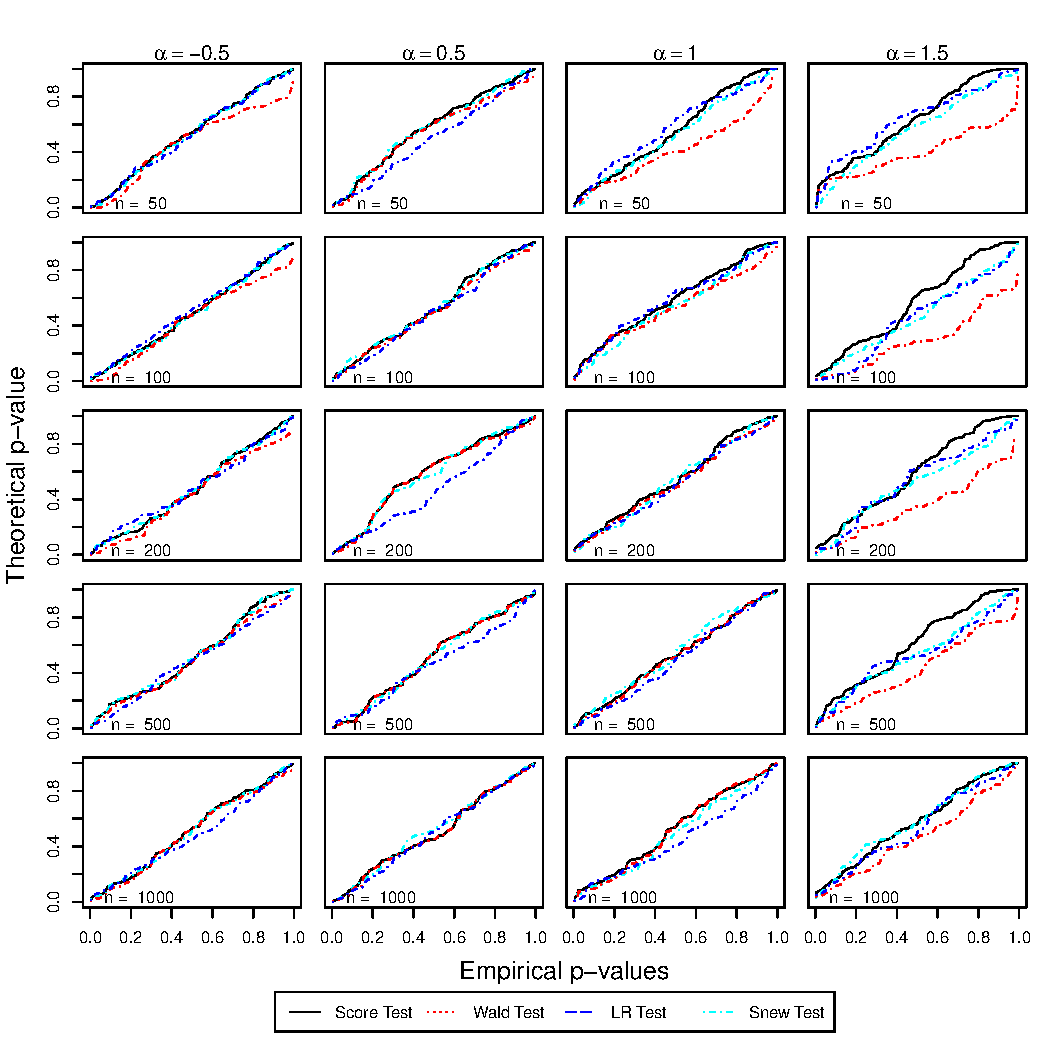
\includegraphics[width=\columnwidth]{./figure/q/q73.pdf}
  \caption{Power plot case3:$\mu=e^{aa-1.45x},x\sim U(0,1)$;cut=7}
\end{figure}

%%%%%%%%%%%%%%%%%%%%%%%%%%%%%%%%%%%%%%%%%%%%%%%%%%%%%%%%%%%%%%%%%%%%%%%%%%%%%%%%%%%

\begin{figure}
  \centering
  % Requires \usepackage{graphicx}
  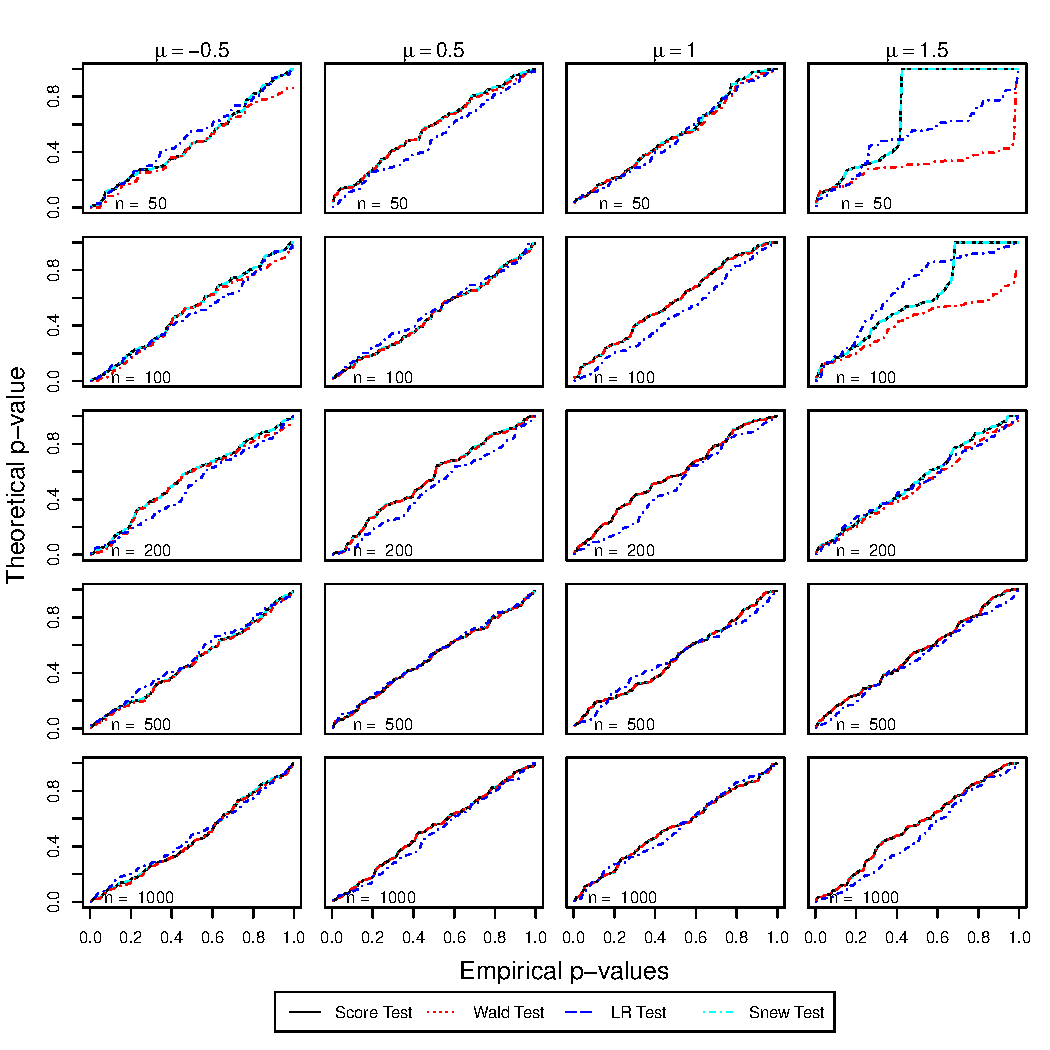
\includegraphics[width=\columnwidth]{./figure/q/q301.pdf}
  \caption{Power plot case1:$\mu=e^{aa}$;cut=30;}
\end{figure}

\begin{figure}
  \centering
  % Requires \usepackage{graphicx}
  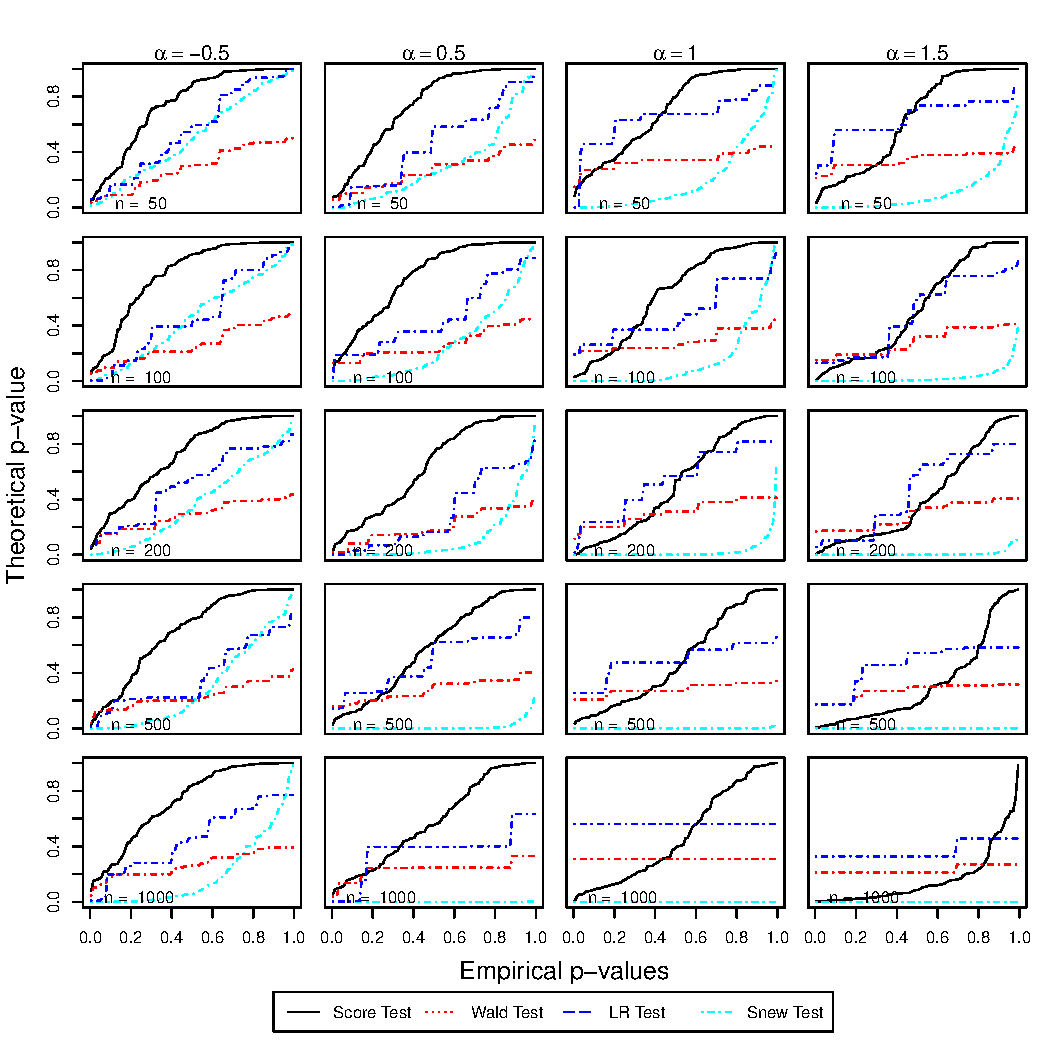
\includegraphics[width=\columnwidth]{./figure/q/q302.pdf}
  \caption{Power plot case2:$\mu=e^{aa-1.45x},x\sim N(0,1)$;cut=30}
\end{figure}

\begin{figure}
  \centering
  % Requires \usepackage{graphicx}
  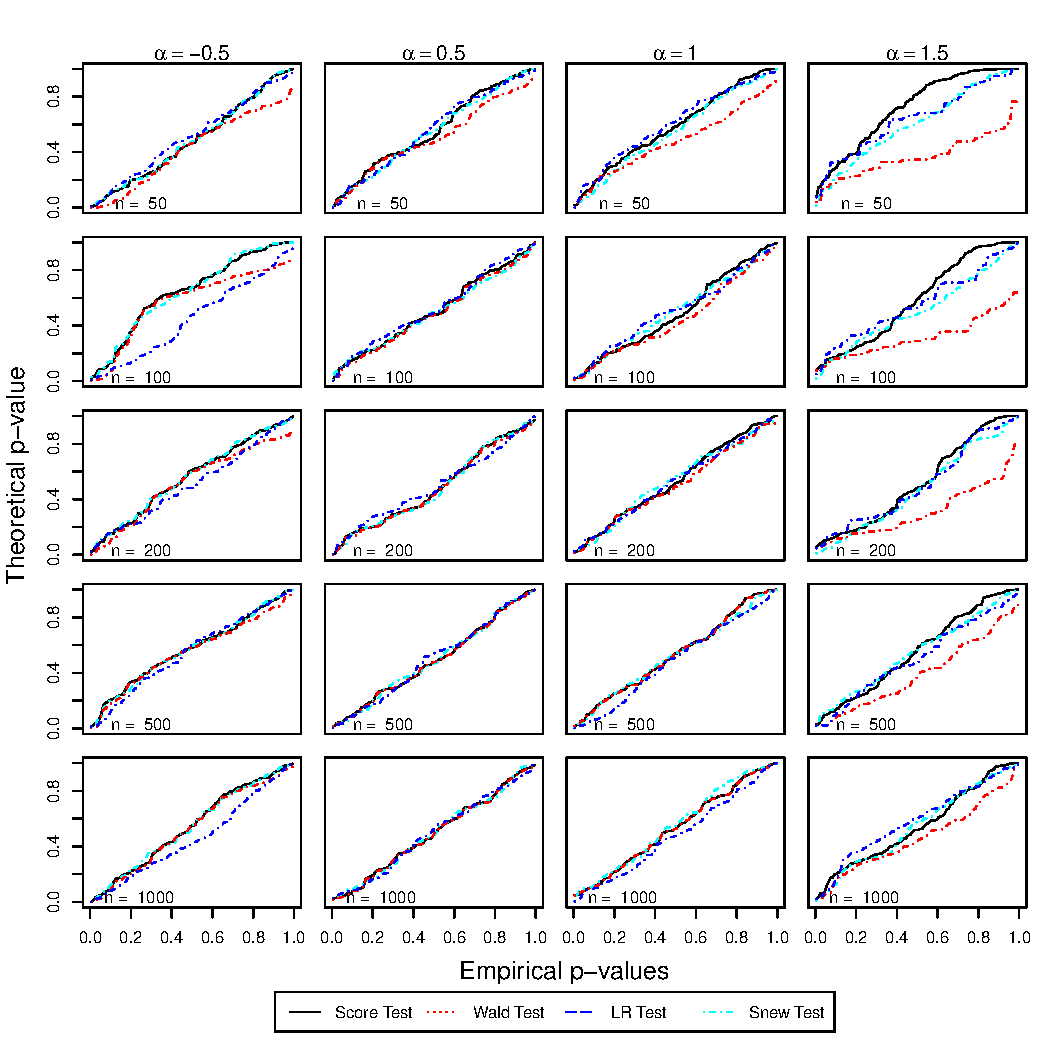
\includegraphics[width=\columnwidth]{./figure/q/q303.pdf}
  \caption{Power plot case3:$\mu=e^{aa-1.45x},x\sim U(0,1)$;cut=30}
\end{figure}




\subsection{Power plot}
\begin{figure}
  \centering
  % Requires \usepackage{graphicx}
  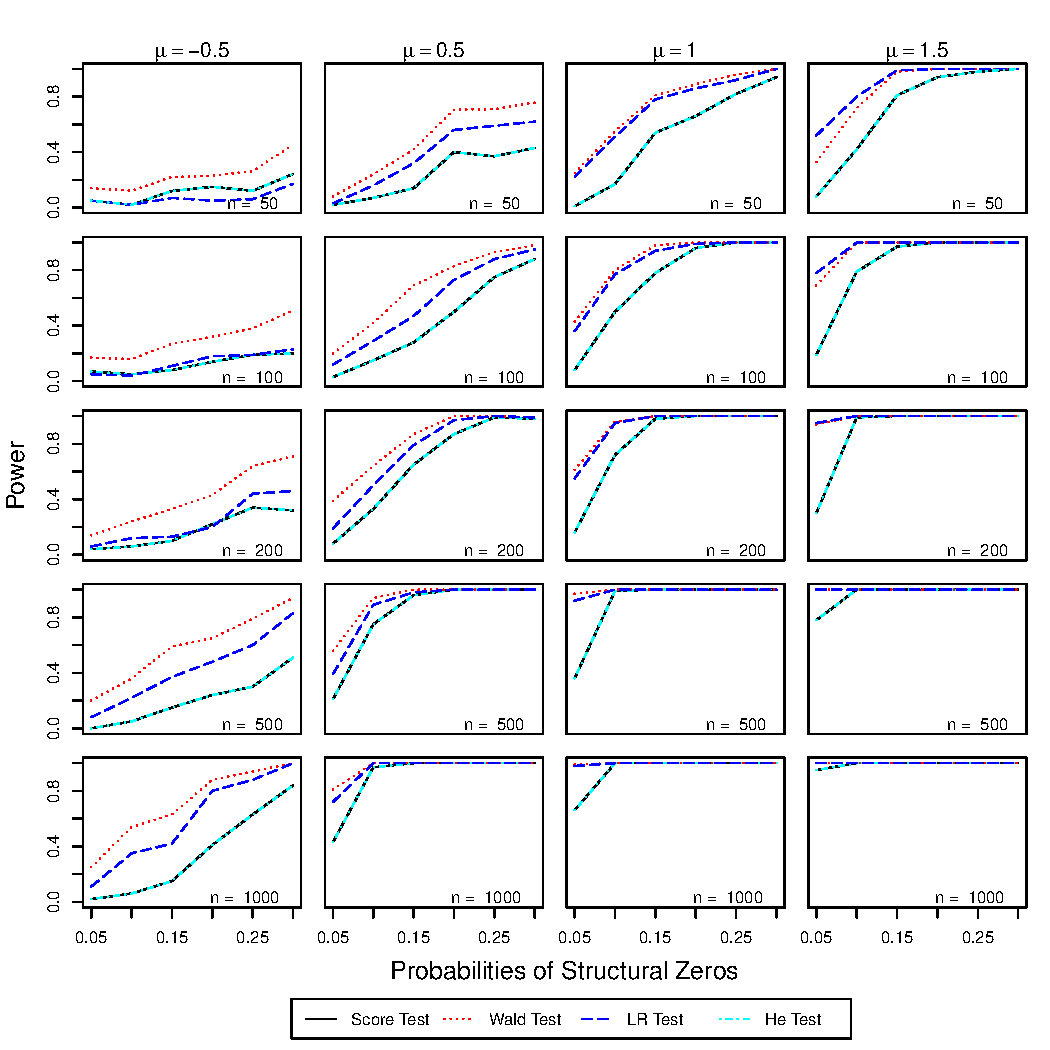
\includegraphics[width=\columnwidth]{./figure/p/p41.pdf}
  \caption{Power plot case1:$\mu=e^{aa},\omega=lp$;cut=4;}
\end{figure}

\begin{figure}
  \centering
  % Requires \usepackage{graphicx}
  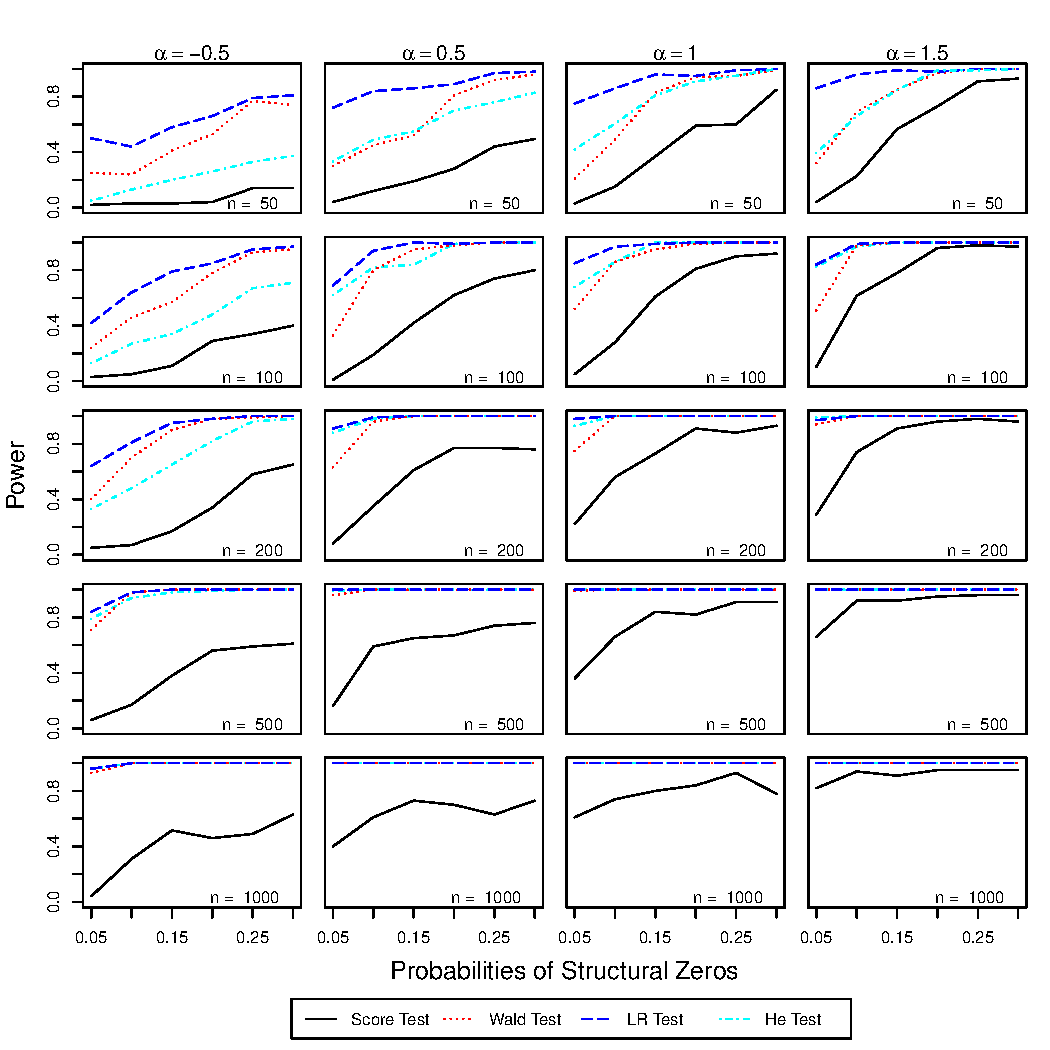
\includegraphics[width=\columnwidth]{./figure/p/p42.pdf}
  \caption{Power plot case2:$\mu=e^{aa-1.45x},\omega=lp,x\sim N(0,1)$;cut=4}
\end{figure}

\begin{figure}
  \centering
  % Requires \usepackage{graphicx}
  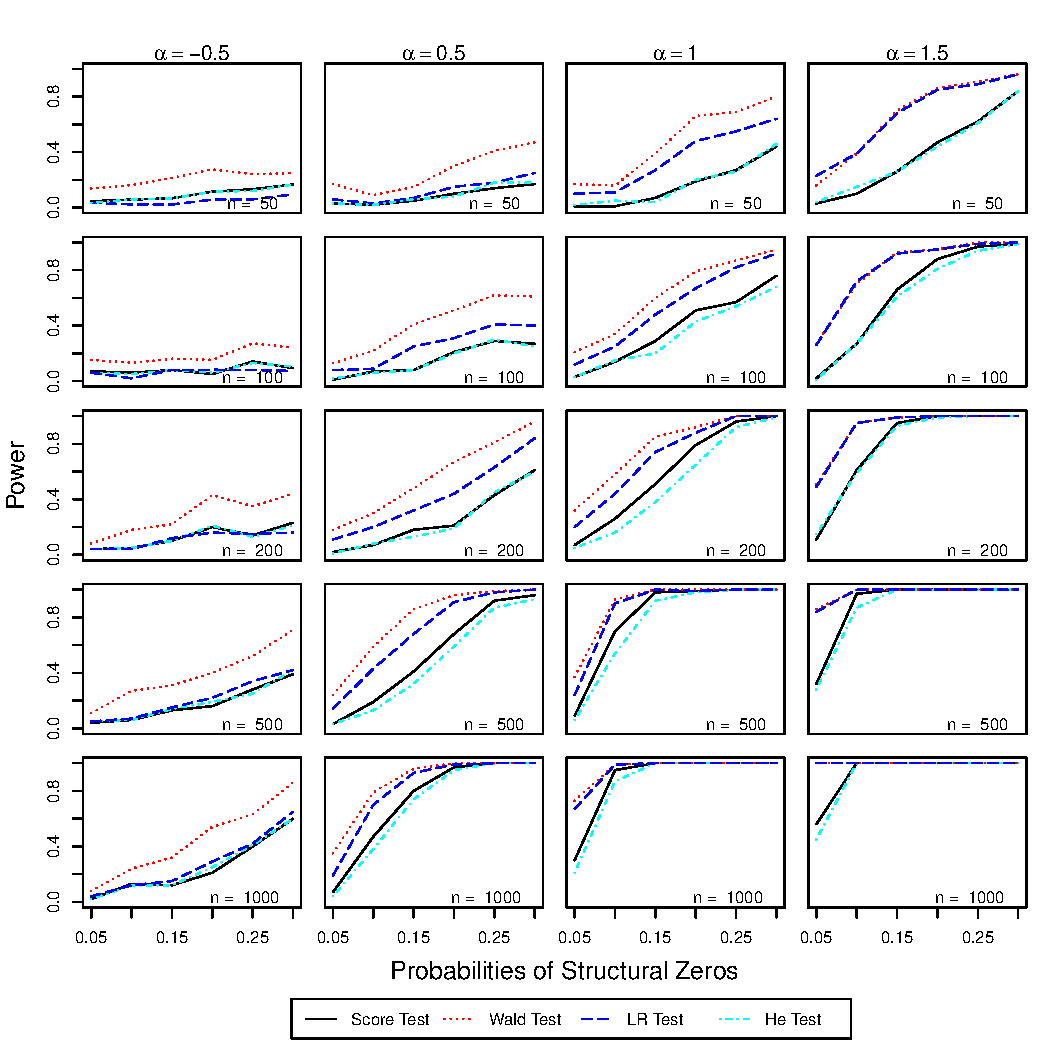
\includegraphics[width=\columnwidth]{./figure/p/p43.pdf}
  \caption{Power plot case3:$\mu=e^{aa-1.45x},\omega=lp,x\sim U(0,1)$;cut=4}
\end{figure}

%%%%%%%%%%%%%%%%%%%%%%%%%%%%%%%%%%%%%%%%%%%%%%%%%%%%%%%%%%%%%%%%%%%%%%%%%%%%%%%%%%%

\begin{figure}
  \centering
  % Requires \usepackage{graphicx}
  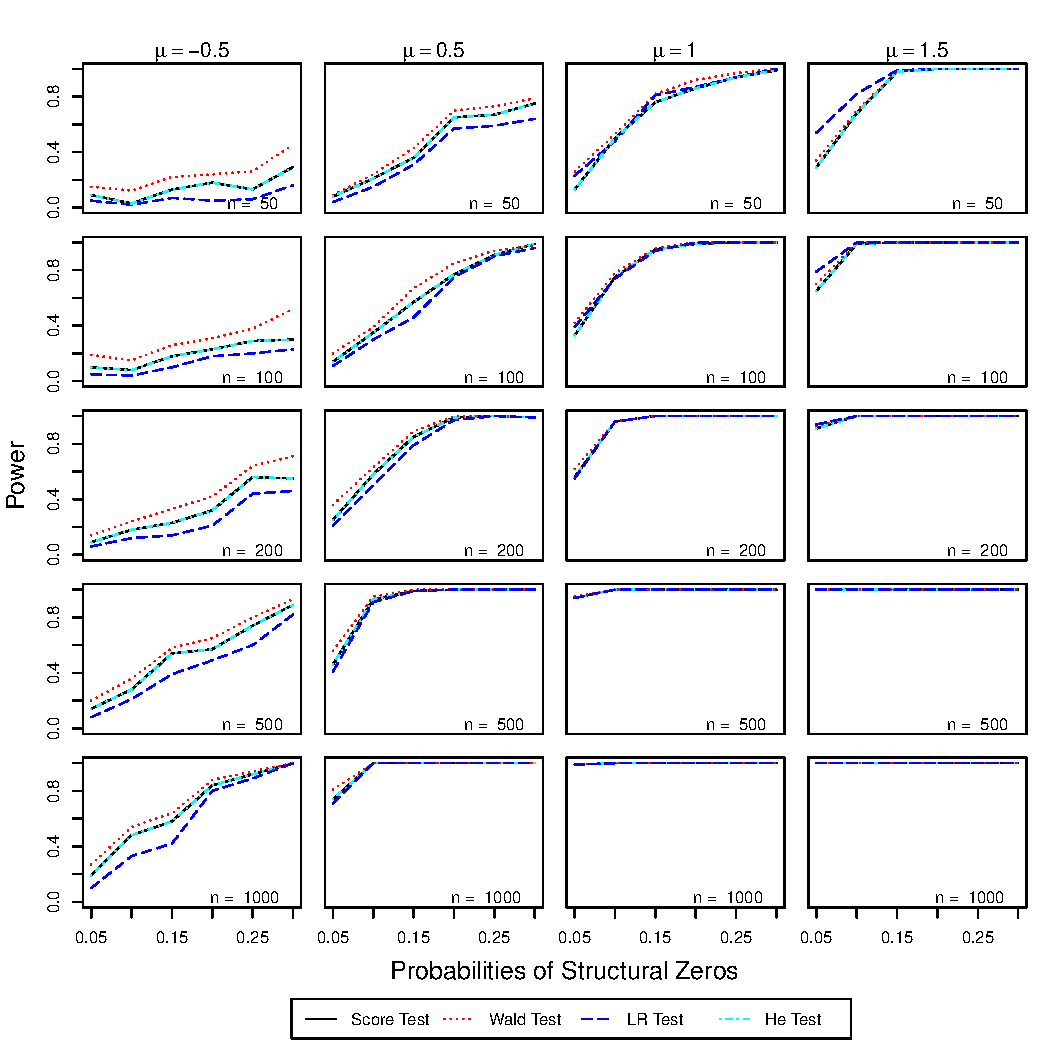
\includegraphics[width=\columnwidth]{./figure/p/p71.pdf}
  \caption{Power plot case1:$\mu=e^{aa},\omega=lp$;cut=7;}
\end{figure}

\begin{figure}
  \centering
  % Requires \usepackage{graphicx}
  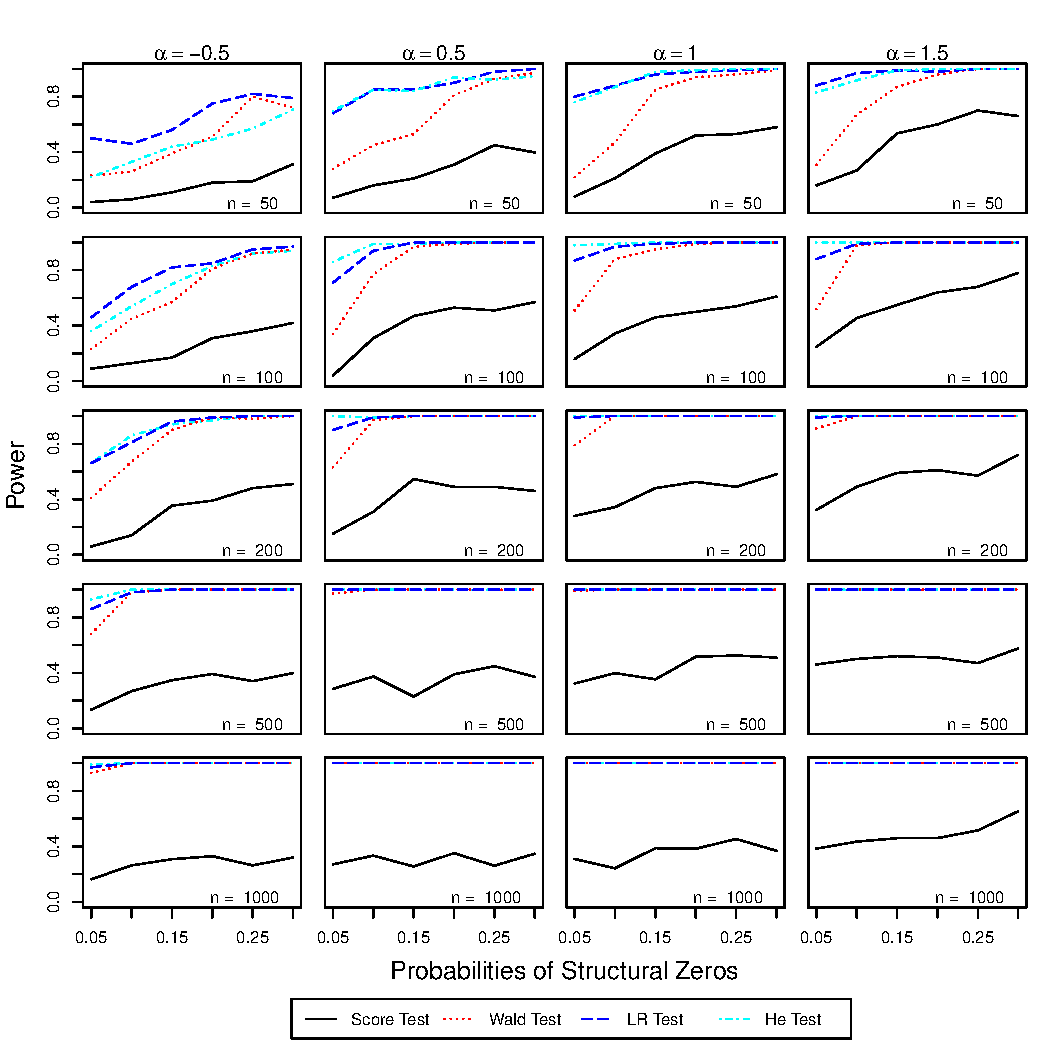
\includegraphics[width=\columnwidth]{./figure/p/p72.pdf}
  \caption{Power plot case2:$\mu=e^{aa-1.45x},\omega=lp,x\sim N(0,1)$;cut=7}
\end{figure}

\begin{figure}
  \centering
  % Requires \usepackage{graphicx}
  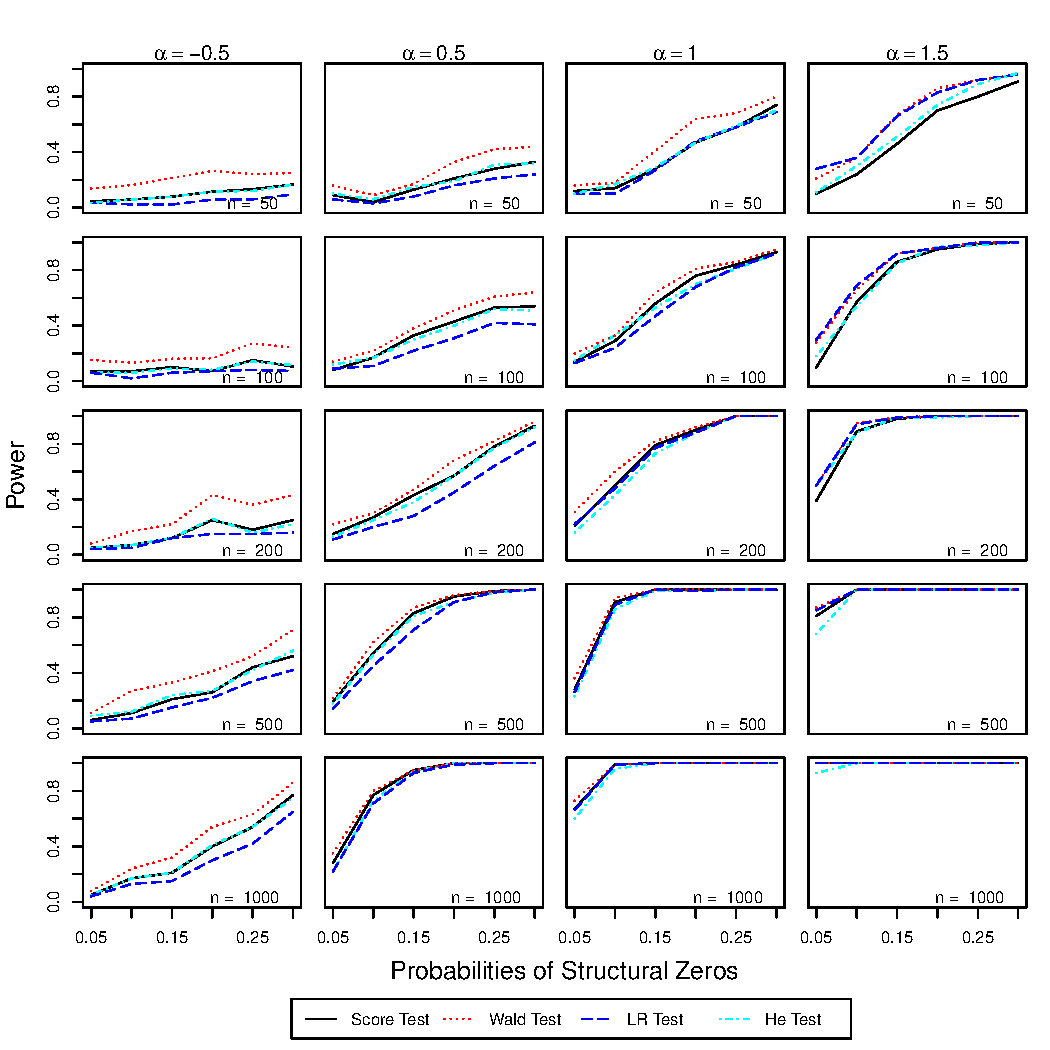
\includegraphics[width=\columnwidth]{./figure/p/p73.pdf}
  \caption{Power plot case3:$\mu=e^{aa-1.45x},\omega=lp,x\sim U(0,1)$;cut=7}
\end{figure}

%%%%%%%%%%%%%%%%%%%%%%%%%%%%%%%%%%%%%%%%%%%%%%%%%%%%%%%%%%%%%%%%%%%%%%%%%%%%%%%%%%%

\begin{figure}
  \centering
  % Requires \usepackage{graphicx}
  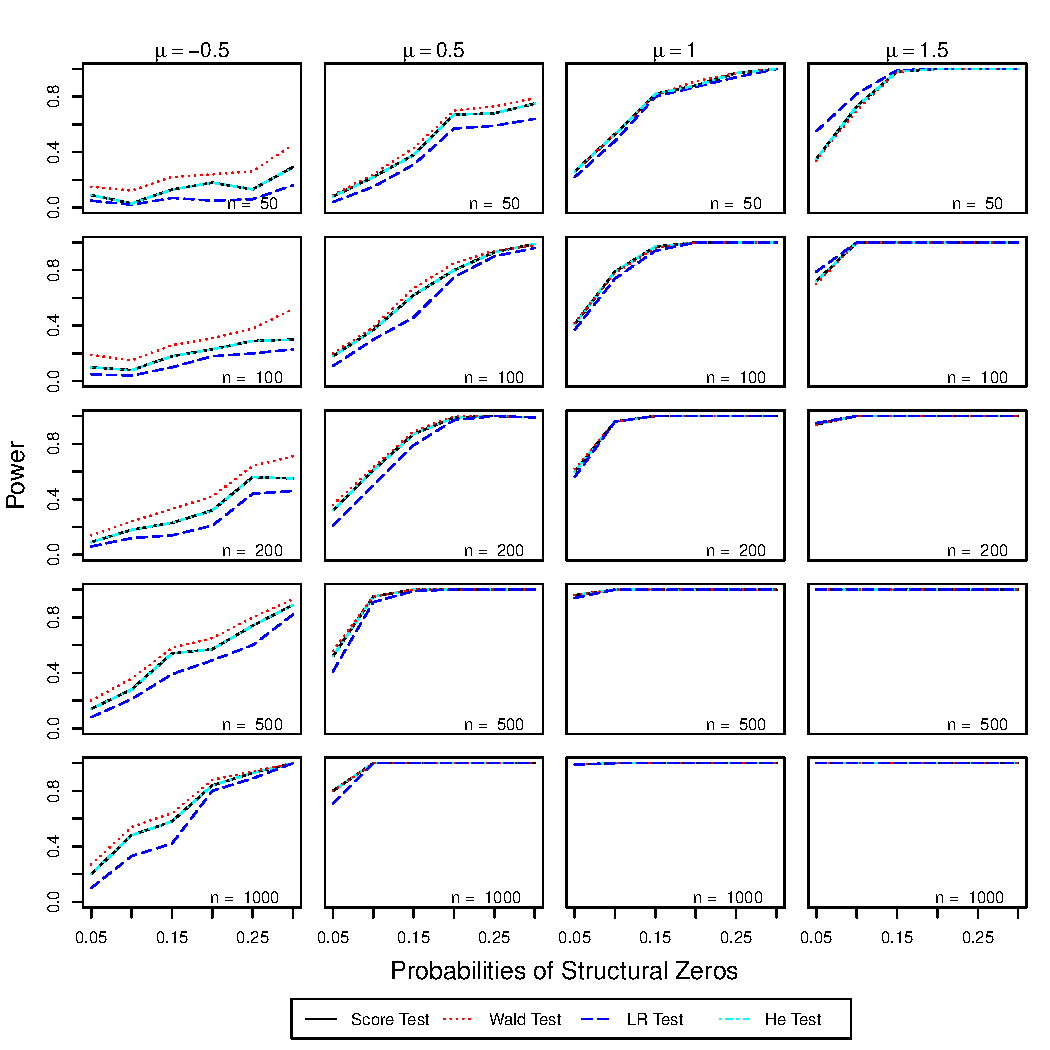
\includegraphics[width=\columnwidth]{./figure/p/p301.pdf}
  \caption{Power plot case1:$\mu=e^{aa},\omega=lp$;cut=30;}
\end{figure}

\begin{figure}
  \centering
  % Requires \usepackage{graphicx}
  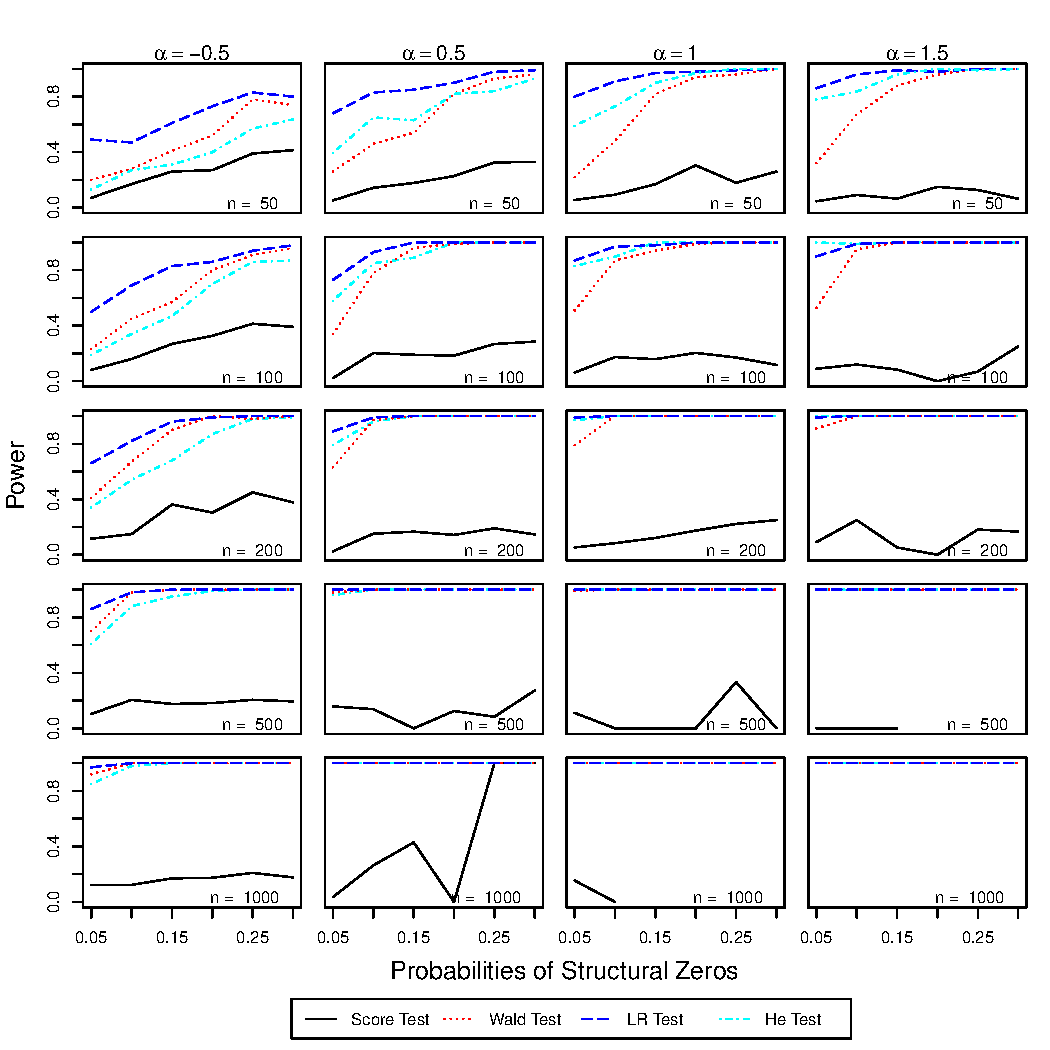
\includegraphics[width=\columnwidth]{./figure/p/p302.pdf}
  \caption{Power plot case2:$\mu=e^{aa-1.45x},\omega=lp,x\sim N(0,1)$;cut=30}
\end{figure}

\begin{figure}
  \centering
  % Requires \usepackage{graphicx}
  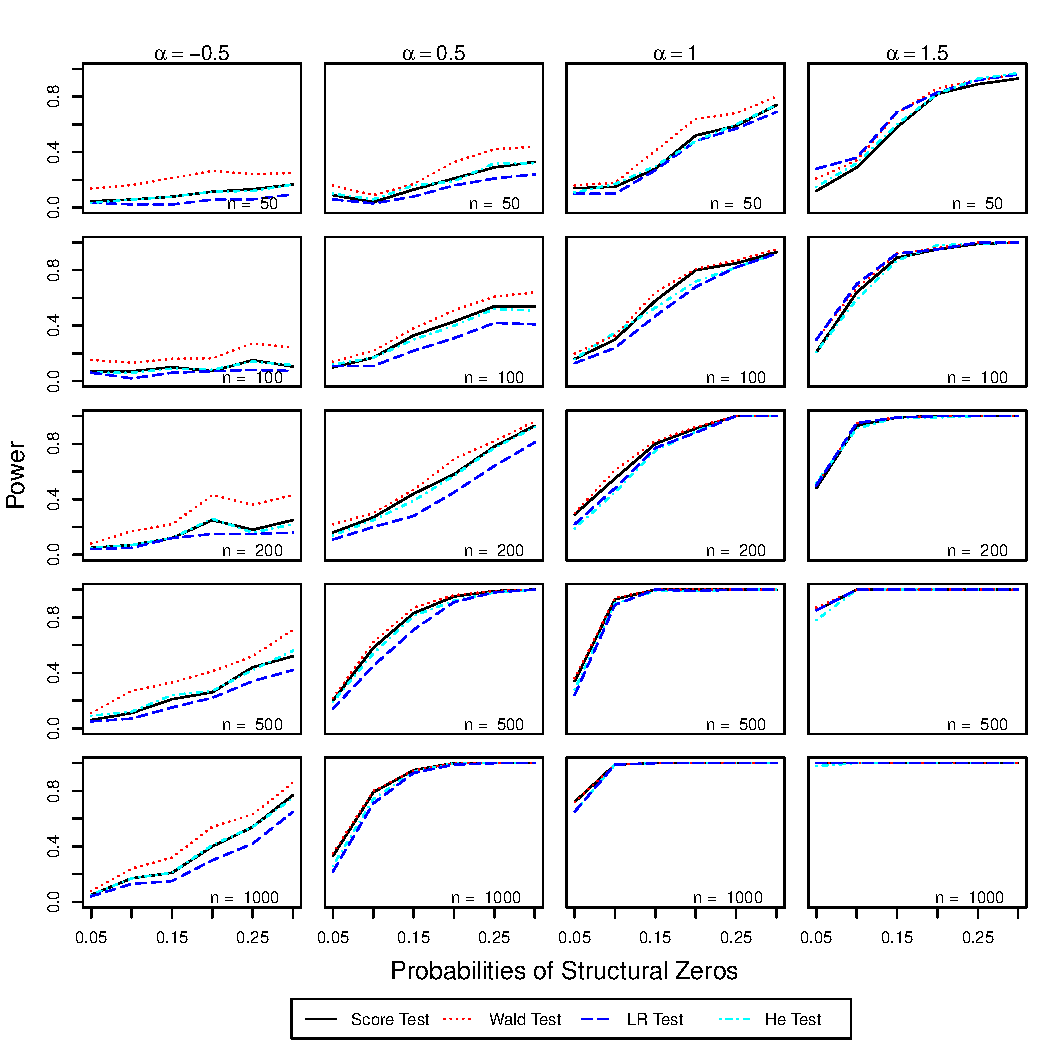
\includegraphics[width=\columnwidth]{./figure/p/p303.pdf}
  \caption{Power plot case3:$\mu=e^{aa-1.45x},\omega=lp,x\sim U(0,1)$;cut=30}
\end{figure}


%%%%%%%%%%%%%%%%%%%%%%%%%%%%%%%%%%%%%%%%%%%%%%%%%%%%%%%%%%%%%%%%%%%%%%%%%%%%%%%%%%%
\end{document}
